\subsection{Spesifikasi Kasus Penggunaan}
	Kasus penggunaan disini dimaksudkan untuk menurunkan kebutuhan fungsional yang telah dispesifikasikan sebelumnya pada tabel \ref{tabel-fungsional} sebelumnya.\\
	Daftar kasus Penggunaan dapat dilihat pada \ref{kasus-penggunaan}.
	
	\LTXtable{\textwidth}{tables/03c/kasus_penggunaan.tex}
	
	Selanjutnya, akan dijabarkan masing-masing Spesifikasi Kasus Penggunaan untuk semua  Kasus Penggunaan yang telah dijabarkan diatas.
	
	\subsubsection{KP01. Manajemen Authentikasi Pengguna}

	Pada kasus penggunaan ini, pengguna dapat memanajemen autentikasi dan pendaftaran ke dalam sistem.\\

	% Login
	\begin{table}[H]
	\centering
\begin{tabular}{|r|p{8cm}|}
		\hline
		\textbf{Kode}                                                    & UC-01.01                                                     \\ \hline
		\textbf{Nama}                                                    & \textbf{Registrasi}                                         \\ \hline
		\textbf{Aktor}                                                   & Pengguna                                                    \\ \hline
		\textbf{Deskripsi}                                               & Pengguna mendaftar ke dalam akun agar masuk ke dalam sistem \\ \hline
		\textbf{Tipe}                                                    & Fungsional                                                  \\ \hline
		\textbf{\textit{Precondition}}
			& Pengguna belum memiliki akun di aplikasi                    \\ \hline
		\textbf{\textit{Postcondition}} 
			& Pengguna sudah memiliki akun terdaftar di aplikasi          \\ \hline
		\multicolumn{2}{|c|}{\textbf{Alur Kejadian Normal}}                                                                            \\ \hline
		\multicolumn{1}{|l|}{}                                           & 
			\begin{enumerate}
				\item Pengguna membuka Halaman Registrasi
				\item \label{uc0101-show1page}Sistem menampilkan halaman yang berisi Form Registrasi
				\item Pengugna mengisi form tersebut
				\item Setelah selesai mengisi, pengugna mengklik tombol "Registrasi"
				\item \label{al-0101-a} Sistem memvalidasi data yang dimasukkan pengguna
				\item Jika data valid, sistem me\textit{redirect} ke halaman \textit{landing page} dalam keadaan sudah terautentikasi \& aun berhasil didaftarkan.
			\end{enumerate}
		\\ \hline
		\multicolumn{2}{|c|}{\textbf{Alur Kejadian Alternatif}}                                                         \\ \hline
		\multicolumn{1}{|l|}{}                                           & \textbf{Data yang dimasukkan pengguna tidak valid}
			\\ \hline
		\multicolumn{1}{|l|}{}                                           & 
			 \begin{itemize}
			 	\item[\ref{al-0101-a}a.] Sistem tidak dapat memvalidasi data yang dimasukkan pengguna.
			 	\item[\ref{al-0101-a}b.] Sistem me\textit{redirect} ke halaman form registrasi (langkah \ref{uc0101-show1page}) dengan \textit{error message}.
			 \end{itemize}
		 \\ \hline
	\end{tabular}
	\caption{Spesifikasi Kasus Penggunaan Registrasi }
	\label{uc01.01}
\end{table}
	
	% Registrasi
	\begin{table}[H]
	\centering
	\begin{tabular}{|r|p{8cm}|}
		\hline
		\textbf{Kode}                                                    & UC-01.02                                                     \\ \hline
		\textbf{Nama}                                                    & \textbf{\textit{Login}}                                         \\ \hline
		\textbf{Aktor}                                                   & Pengguna                                                    \\ \hline
		\textbf{Deskripsi}                                               & Pengguna melakukan \textit{login} agar dapat masuk ke dalam aplikasi dalam keadaan terauthentikasi. \\ \hline
		\textbf{Tipe}                                                    & Fungsional                                                  \\ \hline
		\textbf{\textit{Precondition}}
		& Pengguna masuk ke dalam aplikasi dalam keadaan belum terautentikasi                    \\ \hline
		\textbf{\textit{Postcondition}} 
		& Pengguna masuk ke dalam aplikasi dalam keadaan sudah terautentikasi          \\ \hline
		\multicolumn{2}{|c|}{\textbf{Alur Kejadian Normal}}                                                                            \\ \hline
		\multicolumn{1}{|l|}{}                                           & 
		\begin{enumerate}
			\item Pengguna membuka Halaman Login
			\item \label{uc0102-show1page}Sistem menampilkan halaman Login
			\item Pengguna mengisi halaman sesuai \textit{credential} yang dimiliki
			\item Setelah selesai mengisi, pengguna mengklik tombol "Login"
			\item \label{al-0102-a} Sistem memverifikasi \textit{credential} yang diberikan
			\item Jika data benar, sistem me\textit{redirect} ke halaman \textit{landing page} dalam keadaan sudah terautentikasi.
		\end{enumerate}
		\\ \hline
		\multicolumn{2}{|c|}{\textbf{Alur Kejadian Alternatif}}                                                         \\ \hline
		\multicolumn{1}{|l|}{}                                           & \textbf{Data yang dimasukkan pengguna tidak valid}
		\\ \hline
		\multicolumn{1}{|l|}{}                                           & 
		\begin{itemize}
			\item[\ref{al-0101-a}a.] Sistem tidak dapat memverifikasi \textit{credential} pengguna.
			\item[\ref{al-0101-a}b.] Sistem me\textit{redirect} ke halaman Login (langkah \ref{uc0102-show1page})dengan \textit{error message}.
		\end{itemize}
		\\ \hline
	\end{tabular}
	\caption{Spesifikasi Kasus Penggunaan Login }
	\label{uc0102-tab}
\end{table}
	
	% Konfirmasi Email
	\begin{table}[H]
	\centering
	\begin{tabular}{|r|p{8cm}|}
		\hline
		\textbf{Kode}                                                    & 	UC-01.03                                                     \\ \hline
		\textbf{Nama}                                                    & \textbf{Konfirmasi Email}                                         \\ \hline
		\textbf{Aktor}
			& Pengguna                                                    \\ \hline
		\textbf{Deskripsi}                                               & Pengguna melakukan konfirmasi email agar status akun pengguna menjadi teraktivasi \\ \hline
		\textbf{Tipe}
			& Fungsional                                                  \\ \hline
		\textbf{\textit{Precondition}}
			& Status akun pengguna masih belum terverifikasi \\ \hline
		\textbf{\textit{Postcondition}} 
			&  Status akun pengguna masih sudah	 terverifikasi \\ \hline
		\multicolumn{2}{|c|}{\textbf{Alur Kejadian Normal}}                                                                            \\ \hline
		\multicolumn{1}{|l|}{}                                           & 
			\begin{enumerate}
				\item Pengguna membuka halaman \textit{inbox} email pengguna di \textit{sistem email service} yang mereka gunakan.
				\item pengguna mencari dan membuka email konfirmasi yang dikirimkan oleh Lelangapa
				\item Sistem \textit{email service} pengguna menampilkan isi email konfirmasi, beserta sebuah tombol "Konfirmasi email"
				\item Pengguna mengklik tombol "Konfirmasi Email"
				\item Halaman \textit{browser} akan di\textit{redirect} ke URL konfirmasi email
				\item Sistem menampilkan halaman \textit{landing page} dimana status akun pengguna sudah terverifikasi.
			\end{enumerate}
		\\ \hline
		\multicolumn{2}{|c|}{\textbf{Alur Kejadian Alternatif}}                                                         \\ \hline
		\multicolumn{1}{|l|}{}                                           & -
		\\ \hline
	\end{tabular}
	\caption{Spesifikasi Kasus Penggunaan: Konfirmasi Email}
	\label{uc0103-tab}
\end{table}
	
	\subsubsection{KP02. Manajemen Transaksi Lelang}
\label{kp02}

Pada kasus penggunaan ini, pengguna akan dapat memanajemen transaksi dan penawaran-penawaran yang ia berikan terhadap barang yang terdaftar dalam alikasi.\\

	% Melihat daftar barang yang dilelang
	% Melihat daftar barang yang dilelang

\begin{table}[H]
	\centering
	\caption{Spesifikasi Kasus Penggunaan : Melihat barang yang dilelang}
	\label{uc02.01}
	\begin{tabular}{|r|p{8cm}|}
		\hline
		\textbf{Kode}                                                    & UC-02.01                                                     \\ \hline
		\textbf{Nama}                                                    
			& \textbf{Melihat daftar barang yang dilelang}                                         
			\\ \hline
		\textbf{Aktor}                                                   & Pengguna                                                    \\ \hline
		\textbf{Deskripsi}
			& Pengguna melihat daftar barang yang sedang dilelang
			\\ \hline
		\textbf{Tipe}                                                    
			& Fungsional
			\\ \hline
		\textbf{\textit{Pre Condition}}
			& Sistem belum menampilkan daftar barang yang sedang dilelang
			\\ \hline
		\textbf{\textit{Post Condition}}
			& Sistem menampilkan daftar barang yang sedang dilelang
			\\ \hline
		\multicolumn{2}{|c|}{\textbf{Alur Kejadian Normal}}                                                                            \\ \hline
		\multicolumn{1}{|l|}{}                                           & 
		\begin{enumerate}
			\item Pengguna mengklik \textit{icon} aplikasi di kiri atas halaman
			\item Sistem menampilkan halaman depan yang berisi daftar barang yang sedang dilelang
				  \newline
				  \textit{Ket : Pada halaman depan, ditampilkan barang sesuai dengan kategori berdasarkan waktu dan popularitas, seperti Hot Item (barang yang paling ramai transaksi bidnya), Newest Item, dll.}
		\end{enumerate}
		\\ \hline
		\multicolumn{2}{|c|}{\textbf{Alur Kejadian Alternatif}}                                                         \\ \hline
		\multicolumn{1}{|l|}{}                                           
			& -
		\\ \hline
	\end{tabular}
\end{table}
	
	% Mencari barang yang diinginkan
	% Mencari Barang Lelang

\begin{table}[H]
	\centering
	\begin{tabular}{|r|p{8cm}|}
		\hline
		\textbf{Kode}                                                    
			& UC-02.02                                                     
			\\ \hline
		\textbf{Nama}                                                    
			& \textbf{Mencari Barang Lelang}                                         
			\\ \hline
		\textbf{Aktor}                                                   
			& Pengguna                                                    
			\\ \hline
		\textbf{Deskripsi}
			& Pengguna ingin mencari barang lelang dengan kriteria nama tertentu
			\\ \hline
		\textbf{Tipe}                                                    
			& Fungsional
			\\ \hline
		\textbf{\textit{Pre Condition}}
			& Pengguna menemukan barang lelang yang ia cari dengan kriteria \textit{string}.
			\\ \hline
		\textbf{\textit{Post Condition}}
			& Pengguna menemukan barang lelang yang ia cari dengan kriteria \textit{string} masukan.
			\\ \hline
			\multicolumn{2}{|c|}
			{\textbf{Alur Kejadian Normal}} 
			\\ \hline
		\multicolumn{1}{|l|}{} &
			\begin{enumerate}
				\item Pengguna memasukkan kriteria \textit{string }pencarian di \textit{field} masukan di \textit{Header Bar}
				\item Setelah selesai, pengguna mengklik tombol "Cari"
				\item Sistem mencari barang terdaftar yang sesuai dengan kriteria masukan pengguna
				\item \label{uc0202-a} Jika ketemu, sistem menampilkan halaman "Hasil Pencarian" beserta barang yang sesuai dengan kriteria pengguna.
				\item Pengguna lalu mengklik barang yang sesuai dengan keinginan
				\item Sistem menampilkan detail barang yang sesuai dengan keinginan pengguna
			\end{enumerate}
			\\ \hline
		\multicolumn{2}{|c|}
			{\textbf{Alur Kejadian Alternatif}} 
			\\ \hline
		\multicolumn{1}{|l|}{}                                           
			& \textbf{Tidak ada barang terdaftar dalam sistem yang sesuai dengan kriteria pengguna.}
			\\ \hline
		\multicolumn{1}{|l|}{} & 
			\begin{itemize}
				\item[\ref{uc0202-a}]a. Sistem tidak dapat menemukan barang yang sesuai
				\item[\ref{uc0202-a}]b. Sistem menampilkan "Hasil Pencarian" namun dengan keterangan "Hasil pencarian kosong"
			\end{itemize}
			\\ \hline
	\end{tabular}
	\caption{Spesifikasi Kasus Penggunaan : Mencari Barang Lelang}
	\label{uc02.02}
\end{table}	

	
	% Menawar/melelang barang
		% Menawar/melelang barang
	
	\begin{table}[H]
		\centering
		\caption{Spesifikasi Kasus Penggunaan : Mencari Barang Lelang}
		\label{uc02.03}
		\begin{tabular}{|r|p{8cm}|}
			\hline
			\textbf{Kode}                                                    
			& UC-02.03                                                     
			\\ \hline
			\textbf{Nama}                                                    
			& \textbf{Mencari Barang Lelang}                                         
			\\ \hline
			\textbf{Aktor}                                                   
			& Pengguna                                                    
			\\ \hline
			\textbf{Deskripsi}
			& Pengguna ingin mencari barang lelang dengan kriteria nama tertentu
			\\ \hline
			\textbf{Tipe}                                                    
			& Fungsional
			\\ \hline
			\textbf{\textit{Pre Condition}}
			& Pengguna menemukan barang lelang yang ia cari dengan kriteria \textit{string}.
			\\ \hline
			\textbf{\textit{Post Condition}}
			& Pengguna menemukan barang lelang yang ia cari dengan kriteria \textit{string} masukan.
			\\ \hline
			\multicolumn{2}{|c|}
			{\textbf{Alur Kejadian Normal}}
			\\ \hline
			\multicolumn{1}{|l|}{} & 
			\begin{enumerate}
				\item Pengguna memasukkan kriteria \textit{string }pencarian di \textit{field} masukan di \textit{Header Bar}
				\item Setelah selesai, pengguna mengklik tombol "Cari"
				\item Sistem mencari barang terdaftar yang sesuai dengan kriteria masukan pengguna
				\item \label{uc0202-a} Jika ketemu, sistem menampilkan halaman "Hasil Pencarian" beserta barang yang sesuai dengan kriteria pengguna.
				\item Pengguna lalu mengklik barang yang sesuai dengan keinginan
				\item Sistem menampilkan detail barang yang sesuai dengan keinginan pengguna
			\end{enumerate}
			\\ \hline
			\multicolumn{2}{|c|}
			{\textbf{Alur Kejadian Alternatif}} 
			\\ \hline
			\multicolumn{1}{|l|}{}                                           
			& -
			\\ \hline
		\end{tabular}
	\end{table}	
	
	
	% Melihat riwayat transaksi penawaran harga terhadap barang
	% Melihat Riwayat Penawaran Lelang Barang

\begin{table}[H]
	\centering
	\begin{tabular}{|r|p{8cm}|}
		\hline
		\textbf{Kode}                                                    
		& UC-02.04                                                    
		\\ \hline
		\textbf{Nama}                                                    
		& \textbf{Melihat 3 Riwayat Penawaran Lelang Barang Teratas}                                         
		\\ \hline
		\textbf{Aktor}                                                   
			& Pengguna                                                    
			\\ \hline
		\textbf{Deskripsi}
			& Pengguna ingin melihat riwayat penawaran lelang terhadap barang yang ia daftarkan
			\\ \hline
		\textbf{Tipe}                                                    
			& Fungsional
			\\ \hline
		\textbf{\textit{Pre Condition}}
			& Pengguna menemukan barang lelang yang ia cari dengan kriteria \textit{string}.
			\\ \hline
		\textbf{\textit{Post Condition}}
			& Pengguna menemukan barang lelang yang ia cari dengan kriteria \textit{string} masukan.
			\\ \hline
		\multicolumn{2}{|c|}{\textbf{Alur Kejadian Normal}}
			\\ \hline
		\multicolumn{1}{|l|}{} & 
			\begin{enumerate}
				\item Pengguna membuka halaman "Kelola Barang"
				\item Pengguna mengklik barang yang ingin dilihat informasi riwayat penawaran lelangnya
				\item Sistem menampilkan halaman informasi barang tersebut
				\item Pengguna mengklik tombol "Lihat Penawaran Teratas"
				\item Sistem menampilkan \textit{modal} berisi 3 riwayat penawaran lelang teratas barang tersebut.
				%\item Pengguna memasukkan kriteria \textit{string }pencarian di \textit{field} masukan di \textit{Header Bar}
				%\item \label{uc0202-a} Jika ketemu, sistem menampilkan halaman "Hasil Pencarian" beserta barang yang sesuai dengan kriteria pengguna.
			\end{enumerate}
			\\ \hline
		\multicolumn{2}{|c|}
		{\textbf{Alur Kejadian Alternatif}} 
		\\ \hline
		\multicolumn{1}{|l|}{}                                           
		& -
		\\ \hline
	\end{tabular}
	\caption{Spesifikasi Kasus Penggunaan : Melihat Riwayat Penawaran Lelang Barang}
	\label{uc02.04}
\end{table}	
	
	\subsubsection{KP03. Manajemen Barang Lelang}
\label{kp03}

Pada kasus penggunaan ini, pengguna akan dapat memanajemen barang yang ia daftarkan untuk dilelang, dan melihat proses monitoringnya, seperti yang dipaparkan pada penjelasan berikut.\\

% Mendaftarkan barang untuk dilelang
% Mendaftarkan barang untuk dilelang

\begin{table}[H]
	\centering
\begin{tabular}{|r|p{8cm}|}
		\hline
		\textbf{Kode}                                                    & UC-01.01                                                     \\ \hline
		\textbf{Nama}                                                    & \textbf{Mendaftarkan Barang Lelang}                                         \\ \hline
		\textbf{Aktor}                                                   & Pengguna                                                    \\ \hline
		\textbf{Deskripsi}                                               & Pengguna mendaftarkan barang untuk dilelang di dalam sistem \\ \hline
		\textbf{Tipe}                                                    & Fungsional                                                  \\ \hline
		\textbf{\textit{Precondition}}
			& Barang yang akan dilelang belum terdaftar dalam sistem \\ \hline
		\textbf{\textit{Postcondition}} 
			& Barang yang akan dilelang sudah terdaftar dalam sistem \\ \hline
		\multicolumn{2}{|c|}{\textbf{Alur Kejadian Normal}}                                                                            \\ \hline
		\multicolumn{1}{|l|}{}                                           & 
			\begin{enumerate}
				\item Pengguna membuka Halaman Registrasi
				\item \label{uc0101-show1page}Sistem menampilkan halaman yang berisi Form Registrasi
				\item Pengugna mengisi form tersebut
				\item Setelah selesai mengisi, pengugna mengklik tombol "Registrasi"
				\item \label{al-0101-a} Sistem memvalidasi data yang dimasukkan pengguna
				\item Jika data valid, sistem me\textit{redirect} ke halaman \textit{landing page} dalam keadaan sudah terautentikasi \& aun berhasil didaftarkan.
			\end{enumerate}
		\\ \hline
		\multicolumn{2}{|c|}{\textbf{Alur Kejadian Alternatif}}                                                         \\ \hline
		\multicolumn{1}{|l|}{}                                           & \textbf{Data yang dimasukkan pengguna tidak valid}
			\\ \hline
		\multicolumn{1}{|l|}{}                                           & 
			 \begin{itemize}
			 	\item[\ref{al-0101-a}a.] Sistem tidak dapat memvalidasi data yang dimasukkan pengguna.
			 	\item[\ref{al-0101-a}b.] Sistem me\textit{redirect} ke halaman form registrasi (langkah \ref{uc0101-show1page}) dengan \textit{error message}.
			 \end{itemize}
		 \\ \hline
	\end{tabular}
	\caption{Spesifikasi Kasus Penggunaan Registrasi }
	\label{uc01.01}
\end{table}

% Memperbarui informasi barang yang dilelang
% Memperbarui informasi barang yang dilelang

\begin{table}[H]
	\centering
	\begin{tabular}{|r|p{8cm}|}
		\hline
		\textbf{Kode}                                                    & UC-03.02                                                     \\ \hline
		\textbf{Nama}                                                    & \textbf{Memperbarui informasi barang yang dilelang} \\ \hline
		\textbf{Aktor}                                                   & Pengguna 
			\\ \hline
		\textbf{Deskripsi}                                               & Pengguna memperbarui informasi barang yang sebelumnya sudah terdaftar di dalam sistem 
			 \\ \hline
		\textbf{Tipe}                                                    & Fungsional 
			\\ \hline
		\textbf{\textit{Precondition}}
			& Informasi barang belum diperbarui. \\ \hline
		\textbf{\textit{Postcondition}} 
			& Informasi barang sudah diperbarui. \\ \hline
		\multicolumn{2}{|c|}
			{\textbf{Alur Kejadian Normal}}                                                                            \\ \hline
		\multicolumn{1}{|l|}{}                                           & 
			\begin{enumerate}
				\item Pengguna dalam keadaan terautentikasi, mengklik "Item Anda" -> "Manage Items" pada \textit{navbar} bagian atas halaman.
				\item \label{uc0302-show1page}Sistem menampilkan halaman yang berisi daftar barang yang didaftarkan pengguna.
				\item Pengguna mengklik barang yang ingin diperbarui informasinya
				\item \label{uc0302-show2page}Sistem menampilkan halaman \textit{form} "Perbarui barang".
				\item Pengguna mengisi informasi pembaruan barang di dalam form tersebut.
				\item Setelah selesai, pengguna mengklik tombol "Simpan Pembaruan".
				\item \label{al-0302-a} Sistem memvalidasi data (termasuk file gambar) yang dimasukkan pengguna
				\item Jika data valid, sistem me\textit{redirect} ke halaman "Kelola Barang" dalam keadaan barang baru sudah ditambahkan.
			\end{enumerate}
		\\ \hline
		
		\multicolumn{2}{|c|}{\textbf{Alur Kejadian Alternatif}}                                                         \\ \hline
		\multicolumn{1}{|l|}{}                                           & \textbf{Data barang yang dimasukkan pengguna tidak valid}
			\\ \hline
		\multicolumn{1}{|l|}{}                                           & 
			 \begin{itemize}
			 	\item[\ref{al-0302-a}a.] Sistem tidak dapat memvalidasi data yang dimasukkan pengguna.
			 	\item[\ref{al-0302-a}b.] Sistem me\textit{redirect} ke halaman "Perbarui Barang" (langkah \ref{uc0302-show2page}) dengan \textit{error message}.
			 \end{itemize}
		 \\ \hline
		 \multicolumn{1}{|l|}{}                                           & \textbf{Gambar yang dimasukkan pengguna tidak dapat divalidasi}
		 \\ \hline
		 \multicolumn{1}{|l|}{}                                           & 
		 \begin{itemize}
		 	\item[\ref{al-0302-a}a.] Sistem menampilkan \textit{error modal} berisi peringatan bahwa "Kesalahan saat \textit{upload} gambar, silahkan coba lagi"
		 	\item[\ref{al-0302-a}b.] Sistem me\textit{redirect} ke halaman form "Perbarui Barang" (langkah \ref{uc0301-show2page}) dengan \textit{error message}.
		 \end{itemize}
		 \\ \hline
	\end{tabular}
	\caption{Spesifikasi Kasus Penggunaan : Mendaftarkan Barang Lelang}
	\label{uc03.02}
\end{table}

% Melihat barang yang pernah didaftarkan
% Melihat barang yang pernah didaftarkan

\begin{table}[H]
	\centering
	\begin{tabular}{|r|p{8cm}|}
		\hline
		\textbf{Kode}                                                    & UC-03.03                                                     \\ \hline
		\textbf{Nama}                                                    & \textbf{Melihat Daftar Barang yang Pernah Dilelang} \\ \hline
		\textbf{Aktor}                                                   & Pengguna 
		\\ \hline
		\textbf{Deskripsi}                                               & Pengguna hendak melihat daftar semua barang yang pernah didaftarkan untuk dilelang di dalam sistem.
		\\ \hline
		\textbf{Tipe}                                                    & Fungsional 
		\\ \hline
		\textbf{\textit{Precondition}}
		& Informasi daftar barang belum ditampilkan. \\ \hline
		\textbf{\textit{Postcondition}} 
		& Informasi daftar barang sudah ditampilkan. \\ \hline
		\multicolumn{2}{|c|}
		{\textbf{Alur Kejadian Normal}}                                                                            \\ \hline
		\multicolumn{1}{|l|}{}                                           & 
		\begin{enumerate}
			\item Pengguna dalam keadaan terautentikasi, mengklik "Item Anda" -> "Manage Items" pada \textit{navbar} bagian atas halaman.
			\item \label{uc0302-show1page}Sistem menampilkan halaman yang berisi daftar barang yang didaftarkan pengguna.
		\end{enumerate}
		\\ \hline
		\multicolumn{2}{|c|}{\textbf{Alur Kejadian Alternatif}}                                                         \\ \hline
		\multicolumn{1}{|l|}{}                                           & -
		\\ \hline
	\end{tabular}
	\caption{Spesifikasi Kasus Penggunaan : Melihat Barang yang Pernah Didaftarkan}
	\label{uc03.03}
\end{table}

% Melihat riwayat harga yang ditawarkan pada barang yang dilelang
% Melihat riwayat harga yang ditawarkan pada barang yang dilelang

\begin{table}[H]
	\centering
	\begin{tabular}{|r|p{8cm}|}
		\hline
		\textbf{Kode}                                                    & UC-03.04                                                     \\ \hline
		\textbf{Nama}                                                    & \textbf{Melihat Detail Riwayat Penawaran Harga} \\ \hline
		\textbf{Aktor}                                                   & Pengguna 
		\\ \hline
		\textbf{Deskripsi}                                               & Pengguna hendak melihat daftar semua barang yang pernah didaftarkan dalam sistem.
		\\ \hline
		\textbf{Tipe}                                                    & Fungsional 
		\\ \hline
		\textbf{\textit{Precondition}}
		& Informasi daftar barang belum ditampilkan. \\ \hline
		\textbf{\textit{Postcondition}} 
		& Informasi daftar barang sudah ditampilkan. \\ \hline
		\multicolumn{2}{|c|}
		{\textbf{Alur Kejadian Normal}}                                                                            \\ \hline
		\multicolumn{1}{|l|}{}                                           & 
		\begin{enumerate}
			\item Pengguna dalam keadaan terautentikasi, mengklik "Item Anda" -> "Manage Items" pada \textit{navbar} bagian atas halaman.
			\item Sistem menampilkan halaman yang berisi daftar barang yang didaftarkan pengguna.
			\item Pengguna mengklik barang yang ingin dilihat daftar penawaran harganya
			\item Sistem menampilkan halaman detail informasi barang
			\item Pengguna mengklik tombol "Lihat Riwayat Penawaran"
			\item Sistem menampilkan halaman berisi daftar riwayat penawaran.
		\end{enumerate}
		\\ \hline
		\multicolumn{2}{|c|}{\textbf{Alur Kejadian Alternatif}}                                                         \\ \hline
		\multicolumn{1}{|l|}{}                                           & -
		\\ \hline
	\end{tabular}
	\caption{Spesifikasi Kasus Penggunaan : Melihat Riwayat Penawaran Harga}
	\label{uc03.04}
\end{table}
	
	\subsubsection{KP04. Manajemen Interaksi Antarpengguna}
\label{kp04}
	\begin{figure}[H]
		\centering
		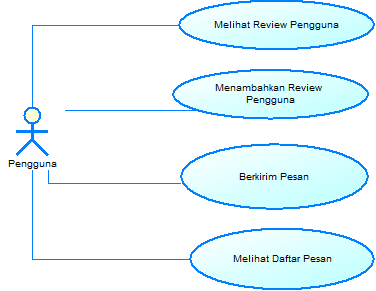
\includegraphics
		[width=\textwidth]
		{images/bab3/usecasediagram/ucd-04.png}
		\caption{Diagram Kasus Penggunaan Manajemen Interaksi Antarpengguna}
		\label{ucd.04}
	\end{figure}
Pada kasus penggunaan ini, pengguna difasilitasi untuk berinteraksi, memberikan \textit{review}/testimoni terhadap pengguna lainnya sesuai dengan keinginan.

	% Melihat review pengguna
	% Melihat review pengguna
	
\begin{table}[H]
	\centering
	\begin{tabular}{|r|p{8cm}|}
		\hline
		\textbf{Kode}                                                    
		& UC-04.01
		\\ \hline
		\textbf{Nama}                                                    
		& \textbf{Melihat \textit{Review} Pengguna} 
		\\ \hline
		
		\textbf{Aktor}  
		& Pengguna 
		\\ \hline
		
		\textbf{Deskripsi}
		& Pengguna ingin melihat \textit{review} pada pengguna tertentu
		\\ \hline
		\textbf{Tipe}                                                    
		& Fungsional 
		\\ \hline
		\textbf{\textit{Precondition}}
		& \textit{Review} pengguna belum ditampilkan
		\\ \hline
		\textbf{\textit{Postcondition}} 
		& \textit{Review} pengguna berhasil ditampilkan
		\\ \hline
		\multicolumn{2}{|c|}
		{\textbf{Alur Kejadian Normal}}                                                                            
		\\ \hline
		\multicolumn{1}{|l|}{} & 
		\begin{enumerate}
			% \item \label{uc0301-show1page}Sistem menampilkan halaman yang berisi form pendaftaran barang
			% \item \label{al-0301-a} Sistem memvalidasi data yang dimasukkan pengguna
			\item Pengguna mengklik \textit{link} profil pengguna
			\item \label{uc0401-a}Sistem menampilkan halaman profil pengguna
			\item Pengguna dapat melihat \textit{review} pengguna di bagian kiri bawah beserta rata-rata \textit{rating} yang diberikan.
		\end{enumerate}
		\\ \hline
		\multicolumn{2}{|c|}{\textbf{Alur Kejadian Alternatif}} \\ \hline
		\multicolumn{1}{|l|}{}                                           
		& -
		\\ \hline
	\end{tabular}
	\caption{Spesifikasi Kasus Penggunaan : Melihat \textit{Review} Pengguna}
	\label{uc04.01}
\end{table}

	
	% Menambahkan Review Pengguna
		% Menambahkan Review Pengguna
	
	
	\begin{table}[H]
		\centering
		\begin{tabular}{|r|p{8cm}|}
			\hline
			\textbf{Kode}                                                    
			& UC-04.02
			\\ \hline
			\textbf{Nama}                                                    
			& \textbf{ Menambahkan Review Pengguna } 
			\\ \hline
			\textbf{Aktor}                                                   
			& Pengguna 
			\\ \hline
			\textbf{Deskripsi}                                               
			& Pengguna ingin menambahkan review dari \textit{transaksi} yang pernah dilakukan.
			\\ \hline
			\textbf{Tipe}
			& Fungsional 
			\\ \hline
			
			\textbf{\textit{Precondition}}
			& Review dari pengguna belum tercatat/tersimpan dalam sistem

			\\ \hline
			
			\textbf{\textit{Postcondition}} 
			& Review dari pengguna berhasil tercatat dalam sistem
			\\ \hline
			
			\multicolumn{2}{|c|}
			{\textbf{Alur Kejadian Normal}}                                                                            
			\\ \hline
			\multicolumn{1}{|l|}{} & 
			\begin{enumerate}
				\item Pengguna mengklik halaman 'Riwayat Transaksi'
				\item Sistem menampilkan halaman Riwayat Transaksi yang pernah dilakukan pengguna
				\item Pengguna mengklik \textit{tab} jenis transaksi yang pernah dilakukan (Beli atau Lelang)
				\item \label{uc0402-show1page}Sistem menampilkan riwayat transaksi sesuai dengan jenis transaksi yang dipilih pengguna
				\item Pengguna mengklik transaksi yang ingin diberikan \textit{review}
				\item \label{al-0402-a}Sistem mengecek apakah \textit{review} sudah pernah diberikan sebelumnya
				\item Sistem menampilkan \textit{modal} berisi \textit{field input} jumlah \textit{rating}
				\item Pengguna mengisi \textit{field} tersebut sesuai jumlah rating yang ingin diberikan
				\item Setelah selesai, pengguna klik 'Next'
				\item Sistem menampilkan \textit{modal} kedua, berisikan \textit{field input} untuk deskripsi \textit{review}
				\item Pengguna mengisikan \textit{field input} sesuai dengan deskripsi yang ingin diberikan
				\item Setelah selesai, pengguna mengklik tombol 'Simpan Review'
				\item \label{al-0402-b}Sistem memvalidasi masukan dari pengguna
				\item Jika tervalidasi, sistem menampilkan modal berisi informasi sukses menyimpan review
				\item Pengguna klik tombol 'Oke'
				\item Sistem menutup \textit{modal} dan kembali ke halaman di poin \cref{uc0402-show1page}
				
				% \item \label{uc0301-show1page}Sistem menampilkan halaman yang berisi form pendaftaran barang
				% \item \label{al-0301-a} Sistem memvalidasi data yang dimasukkan pengguna
			\end{enumerate}
			\\ \hline
			\multicolumn{2}{|c|}{\textbf{Alur Kejadian Alternatif}} \\ \hline
			\multicolumn{1}{|l|}{}                                   \pagebreak        
			& \textbf{Review untuk transaksi yang dipilih sudah pernah diberikan}
			\\ \hline
			\multicolumn{1}{|l|}{}& 
			\begin{itemize}
				\item[\ref{al-0402-a}a.] Sistem mendeteksi bahwa review untuk transaksi tersebut sudah pernah dilakukan
				\item[\ref{al-0402-a}b.] Sistem menampilkan modal berisi informasi bahwa review sudah pernah diberikan, dan \textit{auto-close modal} setelah 4 detik
				\item[\ref{al-0402-a}c.] Sistem menampilkan halaman di poin \cref{uc0402-show1page}
			\end{itemize}
			\\ \hline
			
			\multicolumn{1}{|l|}{}      
			& \textbf{Data masukan pengguna tidak valid}
			\\ \hline
			\multicolumn{1}{|l|}{}& 
			\begin{itemize}
				\item[\ref{al-0402-b}a.] Sistem mendeteksi masukan pengguna tidak valid.
				\item[\ref{al-0402-b}b.] Sistem menampilkan pesan Error berisi \textit{error message}
				\item[\ref{al-0402-b}c.] Sistem menampilkan halaman di poin \cref{uc0402-show1page}
			\end{itemize}
			\\ \hline
		\end{tabular}
		\caption{Spesifikasi Kasus Penggunaan : Memberikan Review Pengguna}
		\label{uc0x.0x-tab}
	\end{table}
		
	% Berikirim pesan
		% Mengirim pesan
	
	
	\begin{table}[H]
		\centering
		\begin{tabular}{|r|p{8cm}|}
			\hline
			\textbf{Kode}
			& UC-04.04
			\\ \hline
			\textbf{Nama}
			& \textbf{ Mengirim Pesan } 
			\\ \hline
			\textbf{Aktor}    
			& Pengguna 
			\\ \hline
			\textbf{Deskripsi}
			& Pengguna akan mengirimkan pesan kepada pengguna lainnya
			\\ \hline
			\textbf{Tipe}
			& Fungsional 
			\\ \hline
			\textbf{\textit{Precondition}}
			& Pesan yang dikirimkan pengguna belum tersimpan pada sistem
			\\ \hline
			\textbf{\textit{Postcondition}} 
			& Pesan yang dikirimkan pengguna berhasil tersimpan pada sistem
			\\ \hline
			\multicolumn{2}{|c|}
			{\textbf{Alur Kejadian Normal}}
			\\ \hline
			\multicolumn{1}{|l|}{} & 
			\begin{enumerate}
				\item Pengguna mengklik \textit{URL} pengguna tujuan yang ingin dikirimi pesan
				\item Sistem menampilkan halaman profil pengguna tujuan
				\item Pengguna mengklik tombol "Kirim Pesan"
				\item Sistem menampilkan halaman percakapan pengguna terhadap tujuan beserta riwayat percakapan pengguna dengan pengguna tujuan
				\item \label{al-0404-ex} Pengguna memasukkan pesan yang ingin dikirimkan pada \textit{field input} yang disediakan
				\item Setelah selesai, pengguna mengklik tombol 'Kirim'
				\item \label{al-0404-a}Sistem mengirim kepada koneksi soket
				\item Jika proses pengiriman kepada soket berhasil dan tidak ada gangguan, sistem kembali menampilkan halaman pengguna dengan informasi pesan yang sudah terkirim muncul di riwayat percakapan pengguna dengan pengguna tujuan
				
				% \item \label{uc0301-show1page}Sistem menampilkan halaman yang berisi form pendaftaran barang
				% \item \label{al-0301-a} Sistem memvalidasi data yang dimasukkan pengguna
			\end{enumerate}
			\\ \hline
			\multicolumn{2}{|c|}{\textbf{Alur Kejadian Alternatif}} \\ \hline
			\multicolumn{1}{|l|}{}                   
			& \textbf{Terjadi masalah teknis sehingga pesan tidak dapat terkirim}
			\\ \hline
			\multicolumn{1}{|l|}{}& 
			\begin{itemize}
				\item[\ref{al-0404-a}a.] Sistem mendapatkan \textit{exception} dari koneksi soket, bahwa pesan tidak dapat tersimpan
				\item[\ref{al-0404-a}b.] Sistem menampilkan kembali halaman pada poin \ref{al-0404-ex}, dengan \textit{modal} berisikan \textit{error message}
			\end{itemize}
			\\ \hline
		\end{tabular}
		\caption{Spesifikasi Kasus Penggunaan : Mengirimkan Pesan}
		\label{uc04.04-tab}
	\end{table}

	% Melihat daftar pesan
		% Melihat dan membaca pesan
	
	
	\begin{table}[H]
		\centering
		\begin{tabular}{|r|p{8cm}|}
			\hline
			\textbf{Kode}
			& UC-04.05
			\\ \hline
			\textbf{Nama}
			& \textbf{Melihat daftar Pesan} 
			\\ \hline
			\textbf{Aktor}    
			& Pengguna 
			\\ \hline
			\textbf{Deskripsi}
			& Pengguna ingin melihat daftar percakapan/ daftar perpesanan yang pernah dilakukan pengguna
			\\ \hline
			\textbf{Tipe}
			& Fungsional 
			\\ \hline
			\textbf{\textit{Precondition}}
			& Daftar percakapan/ daftar perpesanan belum ditampilkan
			\\ \hline
			\textbf{\textit{Postcondition}} 
			& Daftar percakapan/ daftar perpesanan berhasil ditampilkan
			\\ \hline
			\multicolumn{2}{|c|}
			{\textbf{Alur Kejadian Normal}}
			\\ \hline
			\multicolumn{1}{|l|}{} & 
			\begin{enumerate}
				\item Pengguna mengklik tombol 'Conversations' di \textit{navbar} aplikasi
				\item \label{al-0405-a} Sistem menampilkan halaman daftar percakapan pengguna
				\item Sistem memanggil fungsi AJAX untuk meminta data-data percakapan terakhir pengguna
				\item Balasan dari fungsi AJAX di \textit{load} oleh \textit{browser} untuk selanjutnya di\textit{parse} ke dalam HTML
				\item Sistem menampilkan daftar percakapan pengguna
				\item Pengguna mengklik percakapan yang ingin dilihat/dibaca
				\item Sistem menampilkan detail percakapan pengguna dengan pengguna tujuan
			\end{enumerate}
			\\ \hline
		\end{tabular}
		\caption{Spesifikasi Kasus Penggunaan: Melihat \& Membaca Pesan}
		\label{uc04.05}
	\end{table}
	
	\subsubsection{KP05. \textit{Monitoring} Proses Lelang}
\label{kp05}
	\begin{figure}[H]
		\centering
		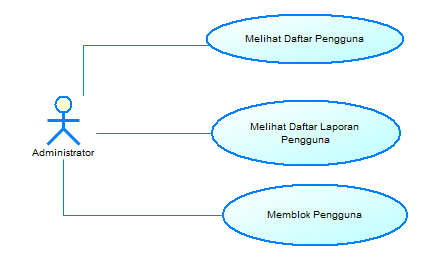
\includegraphics
		[width=\textwidth]
		{images/bab3/buku/usecasediagram/ucd-05.png}
		\caption{Diagram Kasus Penggunaan \textit{Monitoring} Lelang}
		\label{ucd.05}
	\end{figure}
Kasus penggunaan ini seluruhnya digunakan oleh \textit{administrator} aplikasi, dan dilakukan di sistem terpisah.

% Melihat daftar pengguna
	% 
	
	
	\begin{table}[H]
		\centering
		\begin{tabular}{|r|p{8cm}|}
			\hline
			\textbf{Kode}                                                    
			& UC-04.02
			\\ \hline
			\textbf{Nama}                                                    
			& \textbf{ Menambahkan \textit{Review} Pengguna } 
			\\ \hline
			\textbf{Aktor}                                                   
			& Pengguna 
			\\ \hline
			\textbf{Deskripsi}                                               
			& Pengguna ingin menambahkan \textit{review} dari \textit{transaksi} yang pernah dilakukan.
			\\ \hline
			\textbf{Tipe}
			& Fungsional 
			\\ \hline
			
			\textbf{\textit{Precondition}}
			& \textit{Review} dari pengguna belum tercatat/tersimpan dalam sistem

			\\ \hline
			
			\textbf{\textit{Postcondition}} 
			& \textit{Review} dari pengguna berhasil tercatat dalam sistem
			\\ \hline
			
			\multicolumn{2}{|c|}
			{\textbf{Alur Kejadian Normal}}                                                                            
			\\ \hline
			\multicolumn{1}{|l|}{} & 
			\begin{enumerate}
				\item Pengguna mengklik halaman 'Riwayat Transaksi'
				\item Sistem menampilkan halaman Riwayat Transaksi yang pernah dilakukan pengguna
				\item Pengguna mengklik \textit{tab} jenis transaksi yang pernah dilakukan (Beli atau Lelang)
				\item \label{uc0402-show1page}Sistem menampilkan riwayat transaksi sesuai dengan jenis transaksi yang dipilih pengguna
				\item Pengguna mengklik transaksi yang ingin diberikan \textit{review}
				\item \label{al-0402-a}Sistem mengecek apakah \textit{review} sudah pernah diberikan sebelumnya
				\item Sistem menampilkan \textit{modal} berisi \textit{field input} jumlah \textit{rating}
				\item Pengguna mengisi \textit{field} tersebut sesuai jumlah rating yang ingin diberikan
				\item Setelah selesai, pengguna klik 'Next'
				\item Sistem menampilkan \textit{modal} kedua, berisikan \textit{field input} untuk deskripsi \textit{review}
				\item Pengguna mengisikan \textit{field input} sesuai dengan deskripsi yang ingin diberikan
				\item Setelah selesai, pengguna mengklik tombol 'Simpan Review'
				\item \label{al-0402-b}Sistem memvalidasi masukan dari pengguna
				\item Jika tervalidasi, sistem menampilkan modal berisi informasi sukses menyimpan review
				\item Pengguna klik tombol 'Oke'
				\item Sistem menutup \textit{modal} dan kembali ke halaman di poin \ref{uc0402-show1page}
				
				% \item \label{uc0301-show1page}Sistem menampilkan halaman yang berisi form pendaftaran barang
				% \item \label{al-0301-a} Sistem memvalidasi data yang dimasukkan pengguna
			\end{enumerate}
			\\ \hline
			\multicolumn{2}{|c|}{\textbf{Alur Kejadian Alternatif}} \\ \hline
			\multicolumn{1}{|l|}{}                                   \pagebreak        
			& \textbf{Review untuk transaksi yang dipilih sudah pernah diberikan}
			\\ \hline
			\multicolumn{1}{|l|}{}& 
			\begin{itemize}
				\item[\ref{al-0402-a}a.] Sistem mendeteksi bahwa review untuk transaksi tersebut sudah pernah dilakukan
				\item[\ref{al-0402-a}b.] Sistem menampilkan modal berisi informasi bahwa review sudah pernah diberikan, dan \textit{auto-close modal} setelah 4 detik
				\item[\ref{al-0402-a}c.] Sistem menampilkan halaman di poin \ref{uc0402-show1page}
			\end{itemize}
			\\ \hline
			
			\multicolumn{1}{|l|}{}      
			& \textbf{Data masukan pengguna tidak valid}
			\\ \hline
			\multicolumn{1}{|l|}{}& 
			\begin{itemize}
				\item[\ref{al-0402-b}a.] Sistem mendeteksi masukan pengguna tidak valid.
				\item[\ref{al-0402-b}b.] Sistem menampilkan pesan Error berisi \textit{error message}
				\item[\ref{al-0402-b}c.] Sistem menampilkan halaman di poin \ref{uc0402-show1page}
			\end{itemize}
			\\ \hline
		\end{tabular}
		\caption{Spesifikasi Kasus Penggunaan : Memberikan \textit{Review} Pengguna}
		\label{uc04.02}
	\end{table}

% Melihat daftar laporan pengguna
	% Menambahkan Review Pengguna
	
	
	\begin{table}[H]
		\centering
		\caption{Spesifikasi Kasus Penggunaan : Memberikan \textit{Review} Pengguna}
		\label{uc04.02}
		\begin{tabular}{|r|p{8cm}|}
			\hline
			\textbf{Kode}                                                    
			& UC-04.02
			\\ \hline
			\textbf{Nama}                                                    
			& \textbf{ Menambahkan \textit{Review} Pengguna } 
			\\ \hline
			\textbf{Aktor}                                                   
			& Pengguna 
			\\ \hline
			\textbf{Deskripsi}                                               
			& Pengguna ingin menambahkan \textit{review} dari \textit{transaksi} yang pernah dilakukan.
			\\ \hline
			\textbf{Tipe}
			& Fungsional 
			\\ \hline
			
			\textbf{\textit{Precondition}}
			& \textit{Review} dari pengguna belum tercatat/tersimpan dalam sistem \\ \hline
			
			\textbf{\textit{Postcondition}} 
			& \textit{Review} dari pengguna berhasil tercatat dalam sistem
			\\ \hline
			
			\multicolumn{2}{|c|}
			{\textbf{Alur Kejadian Normal}}                                                                            
			\\ \hline
			\multicolumn{1}{|l|}{} & 
			\begin{enumerate}
				\item Pengguna mengklik halaman 'Riwayat Transaksi'
				\item Sistem menampilkan halaman Riwayat Transaksi yang pernah dilakukan pengguna
				\item Pengguna mengklik \textit{tab} jenis transaksi yang pernah dilakukan (Beli atau Lelang)
				\item \label{uc0402-show1page}Sistem menampilkan riwayat transaksi sesuai dengan jenis transaksi yang dipilih pengguna
				\item Pengguna mengklik transaksi yang ingin diberikan \textit{review}
				\item \label{al-0402-a}Sistem mengecek apakah \textit{review} sudah pernah diberikan sebelumnya, lalu menampilkan form penilaian selanjutnya.
				\item Pengguna memasukkan jumlah \textit{rating} dan deskripsi \textit{rating}, lalu klik 'Simpan Review'
				\item \label{al-0402-b}Sistem memvalidasi masukan, jika valid sistem mengembalikan modal status sukses.				
				% \item \label{uc0301-show1page}Sistem menampilkan halaman yang berisi form pendaftaran barang
				% \item \label{al-0301-a} Sistem memvalidasi data yang dimasukkan pengguna
			\end{enumerate}
			\\ \hline
			\multicolumn{2}{|c|}{\textbf{Alur Kejadian Alternatif}} \\ \hline
			\multicolumn{1}{|l|}{}                                   \pagebreak        
			& -
			\\ \hline
		\end{tabular}
	\end{table}

% Memblock pengguna
	% Melaporkan Barang
	
	
	\begin{table}[H]
		\centering
		\begin{tabular}{|r|p{8cm}|}
			\hline
			\textbf{Kode}                                                    
			& UC-04.03
			\\ \hline
			\textbf{Nama}
			
			& \textbf{Melaporkan Barang} 
			\\ \hline
			\textbf{Aktor}                                                   
			& Pengguna 
			\\ \hline
			\textbf{Deskripsi}                                               
			& Pengguna ingin melaporkan barang yang dianggap melanggar aturan/tidak pantas diperjualbelikan
			\\ \hline
			\textbf{Tipe}                                                    
			& Fungsional 
			\\ \hline
			\textbf{\textit{Precondition}}
			& Laporan dari pengguna belum tersimpan dalam sistem
			\\ \hline
			\textbf{\textit{Postcondition}} 
			& Laporan dari pengguna berhasil tersimpan dalam sistem
			\\ \hline
			\multicolumn{2}{|c|}
			{\textbf{Alur Kejadian Normal}}                                                                            
			\\ \hline
			\multicolumn{1}{|l|}{} & 
			\begin{enumerate}
				\item Pengguna mengklik barang yang ingin dilaporkan
				\item \label{uc0403-1page} Sistem menampilkan halaman informasi barang
				\item Pengguna mengklik tombol "Laporkan Barang"
				\item Sistem menampilkan \textit{modal} berisi \textit{input field} laporan
				\item Pengguna mengisi \textit{fields} tersebut sesuai dengan konten laporan yang ingin disampaikan
				\item \label{uc0403-modal}Setelah selesai, pengguna mengklik tombol "Laporkan"
				\item Sistem mengecek dan memvalidasi masukan pengguna
				\item Jika valid, sistem akan menampilkan \textit{modal} Sukses Menyimpan Laporan
				\item Sistem me\textit{redirect} pengguna kembali ke halaman di \ref{uc0403-1page}
				% \item \label{uc0301-show1page}Sistem menampilkan halaman yang berisi form pendaftaran barang
				% \item \label{al-0301-a} Sistem memvalidasi data yang dimasukkan pengguna
			\end{enumerate}
			\\ \hline
			\multicolumn{2}{|c|}{\textbf{Alur Kejadian Alternatif}} \\ \hline
			\multicolumn{1}{|l|}{}      
			& \textbf{Data masukan laporan pengguna tidak valid}
			\\ \hline
			\multicolumn{1}{|l|}{}& 
			\begin{itemize}
				\item[\ref{al-0402-b}a.] Sistem mendeteksi masukan pengguna tidak valid.
				\item[\ref{al-0402-b}c.] Sistem menampilkan kembali modal di poin \ref{uc0403-modal} beserta dengan \textit{error message}
			\end{itemize}
			\\ \hline
		\end{tabular}
		\caption{Spesifikasi Kasus Penggunaan : Melaporkan Barang}
		\label{uc04.03-tab}
	\end{table}
	
	\subsubsection{KP05. Manajemen Voucher}
\label{kp05}

	\begin{figure}[H]
		\centering
		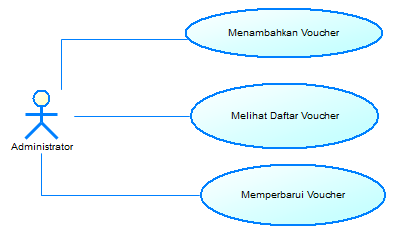
\includegraphics
		[width=\textwidth]
		{images/bab3/usecasediagram/ucd-06.png}
		\caption{Diagram Kasus Penggunaan Manajemen Kupon}
		\label{ucd.06}
	\end{figure}
	Kasus penggunaan ini seluruhnya digunakan oleh \textit{administrator} aplikasi dan dilakukan di sistem terpisah. Kasus penggunaan ditujukan untuk mempermudah \textit{administrator} dalam memanajemen voucher/kupon yang dibagikan oleh pengguna.

	% Menambahkan voucher
		% Memasukkan kupon
	
	\begin{table}[H]
		\centering
		\begin{tabular}{|r|p{8cm}|}
			\hline
			\textbf{Kode}
			& UC-05.01
			\\ \hline
			\textbf{Nama}
			& \textbf{Menambahkan Kupon} 
			\\ \hline
			\textbf{Aktor}    
			& Administrator 
			\\ \hline
			\textbf{Deskripsi}
			& Administrator ingin menggunakan kupon/voucher yang ia miliki untuk pada sebuah transaksi
			\\ \hline
			\textbf{Tipe}
			& Fungsional 
			\\ \hline
			\textbf{\textit{Precondition}}
			& Kupon baru belum berhasil tersimpan di sistem
			\\ \hline
			\textbf{\textit{Postcondition}} 
			& Kupon baru berhasil tersimpan di sistem
			\\ \hline
			\multicolumn{2}{|c|}
			{\textbf{Alur Kejadian Normal}}
			\\ \hline
			\multicolumn{1}{|l|}{} & 
			\begin{enumerate}
				\item Administrator membuka halaman 'Tambah Kupon'
				\item Sistem menampilkan halaman form Tambah Kupon
				\item Administrator memasukkan informasi kupon baru yang akan ditambahkan
				\item Sistem mengecek permintaan penggunaan kupon,jika permintaan dapat diverifikasi dan valid, sistem me\textit{redirect} ke halaman manajemen kupon.
				% \item \label{uc0301-show1page}Sistem menampilkan halaman yang berisi form pendaftaran barang
				% \item \label{al-0301-a} Sistem memvalidasi data yang dimasukkan pengguna
			\end{enumerate}
			\\ \hline
			\multicolumn{2}{|c|}{\textbf{Alur Kejadian Alternatif}} \\ \hline
			\multicolumn{1}{|l|}{}                   
			& -
			\\ \hline
		\end{tabular}
		\caption{Spesifikasi Kasus Penggunaan : Menambahkan Kupon}
		\label{uc06.01}
	\end{table}
	
	% Melihat daftar voucher
		% Memasukkan kupon
	
	\begin{table}[H]
		\centering
		\begin{tabular}{|r|p{8cm}|}
			\hline
			\textbf{Kode}
			& UC-05.02
			\\ \hline
			\textbf{Nama}
			& \textbf{Memasukkan Kupon pada Transaksi} 
			\\ \hline
			\textbf{Aktor}    
			& Pengguna 
			\\ \hline
			\textbf{Deskripsi}
			& Pengguna ingin menggunakan kupon/voucher yang ia miliki untuk pada sebuah transaksi
			\\ \hline
			\textbf{Tipe}
			& Fungsional 
			\\ \hline
			\textbf{\textit{Precondition}}
			& Pengguna belum berhasil men\textit{submit} kode kupon ke dalam transaksi barang
			\\ \hline
			\textbf{\textit{Postcondition}} 
			& Pengguna berhasil men\textit{submit} kode kupon ke dalam transaksi barang
			\\ \hline
			\multicolumn{2}{|c|}
			{\textbf{Alur Kejadian Normal}}
			\\ \hline
			\multicolumn{1}{|l|}{} & 
			\begin{enumerate}
				\item Pengguna membuka halaman 'Riwayat Transaksi Lelang'
				\item Sistem menampilkan halaman Riwayat Transaksi Lelang pengguna
				\item Pengguna mengklik tombol 'Masukkan Kupon' pada transaksi yang diinginkan
				\item Sistem mengecek permintaan penggunaan kupon
				\item Jika permintaan dapat diverifikasi dan valid, sistem menampilkan \textit{modal} berisi \textit{input field} kupon
				\item Pengguna memasukkan kupon yang ingin dimasukkan, lalu mengklik tombol 'Submit'
				\item Sistem memvalidasi kupon voucher dan status barang
				\item Jika valid, sistem menerapkan penggunaan kupon ke dalam transaksi barang
				\item Sistem lalu menampilkan \textit{modal} yang berisi informasi sukses penggunaan kupon pada transaksi
				% \item \label{uc0301-show1page}Sistem menampilkan halaman yang berisi form pendaftaran barang
				% \item \label{al-0301-a} Sistem memvalidasi data yang dimasukkan pengguna
			\end{enumerate}
			\\ \hline
			\multicolumn{2}{|c|}{\textbf{Alur Kejadian Alternatif}} \\ \hline
			\multicolumn{1}{|l|}{}                   
			& -
			\\ \hline
		\end{tabular}
		\caption{Spesifikasi Kasus Penggunaan : Mendaftarkan Barang Lelang}
		\label{uc04.06}
	\end{table}
	
	% Memperbarui Voucher
		% Memasukkan kupon
	
	\begin{table}[H]
		\centering
		\begin{tabular}{|r|p{8cm}|}
			\hline
			\textbf{Kode}
			& UC-05.01
			\\ \hline
			\textbf{Nama}
			& \textbf{Memperbarui Kupon} 
			\\ \hline
			\textbf{Aktor}    
			& Administrator 
			\\ \hline
			\textbf{Deskripsi}
			& Administrator ingin memperbarui kupon
			\\ \hline
			\textbf{Tipe}
			& Fungsional 
			\\ \hline
			\textbf{\textit{Precondition}}
			& Kupon belum diperbarui
			\\ \hline
			\textbf{\textit{Postcondition}} 
			& Kupon berhasil diperbarui
			\\ \hline
			\multicolumn{2}{|c|}
			{\textbf{Alur Kejadian Normal}}
			\\ \hline
			\multicolumn{1}{|l|}{} & 
			\begin{enumerate}
				\item Administrator membuka halaman 'Manajemen Kupon'
				\item Sistem menampilkan halaman form Edit Kupon pada sesuai dengan data kupon yang ingin diperbarui
				\item Administrator memasukkan informasi kupon baru yang ingin ditambahkan, lalu ketik tombol "Submit"
				\item Sistem mengecek informasi baru kupon kupon,lalu sistem me\textit{redirect} ke halaman manajemen kupon dengan info sukses.
				% \item \label{uc0301-show1page}Sistem menampilkan halaman yang berisi form pendaftaran barang
				% \item \label{al-0301-a} Sistem memvalidasi data yang dimasukkan pengguna
			\end{enumerate}
			\\ \hline
			\multicolumn{2}{|c|}{\textbf{Alur Kejadian Alternatif}} \\ \hline
			\multicolumn{1}{|l|}{}                   
			& -
			\\ \hline
		\end{tabular}
		\caption{Spesifikasi Kasus Penggunaan : Menambahkan Kupon}
		\label{uc06.03}
	\end{table}







